\documentclass[week2]{csse1001}

\title{CSSE1001 Week 7 Practicals}
 
\begin{document}

\begin{frame} 
\maketitle
\end{frame}

\section{Assignment 1 Common Pitfalls}

\begin{topic}{Duplicated code in decrypt}
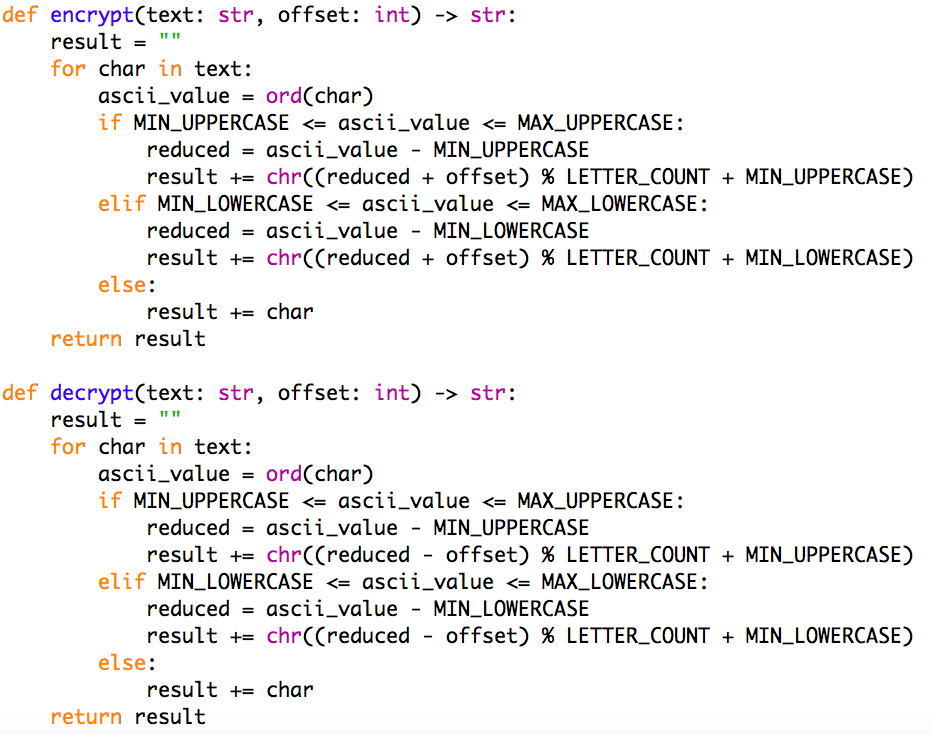
\includegraphics[width=0.9\textwidth]{a1pitfalls/baddecrypt}
\end{topic}

\begin{topic}{This is better}
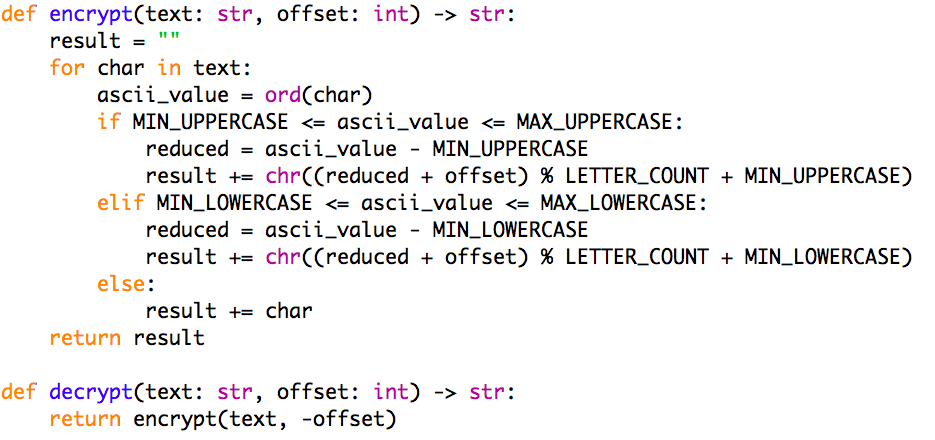
\includegraphics[width=\textwidth]{a1pitfalls/gooddecrypt}
\end{topic}

\begin{topic}{Print vs return}
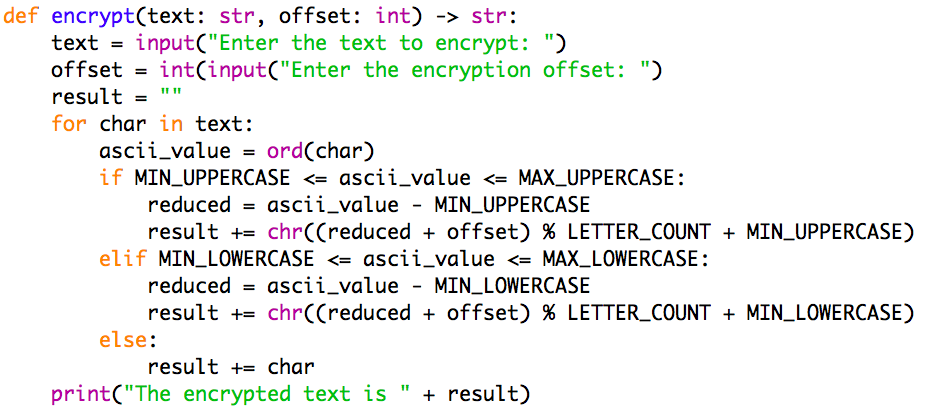
\includegraphics[width=\textwidth]{a1pitfalls/pvr}
\end{topic}

\begin{topic}{For vs while}
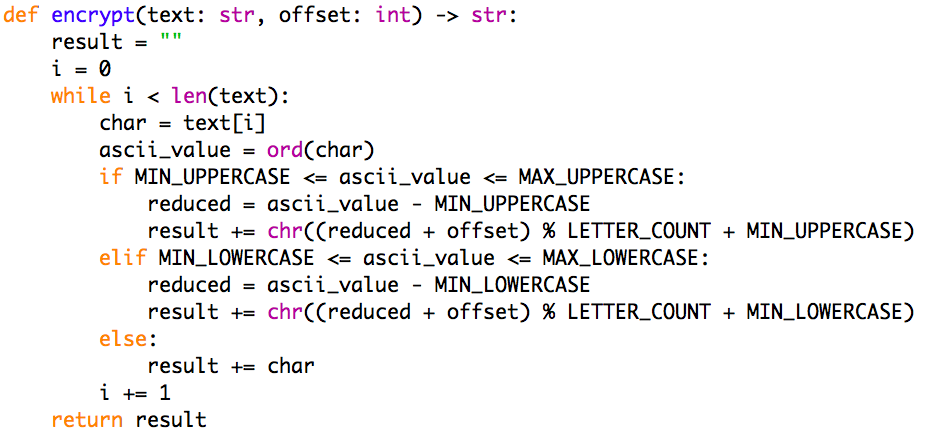
\includegraphics[width=\textwidth]{a1pitfalls/while}
\end{topic}

\begin{topic}{Magic numbers}
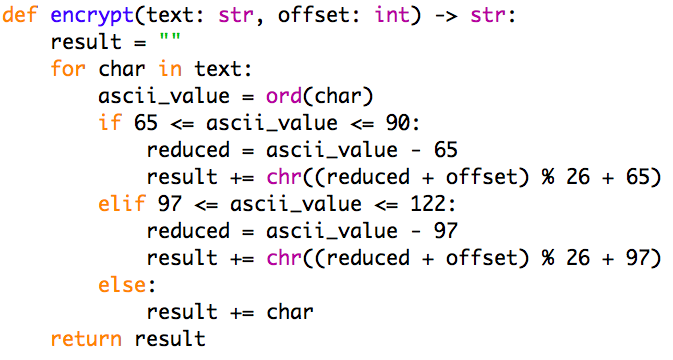
\includegraphics[width=\textwidth]{a1pitfalls/magic}
\end{topic}

\begin{topic}{This is better}
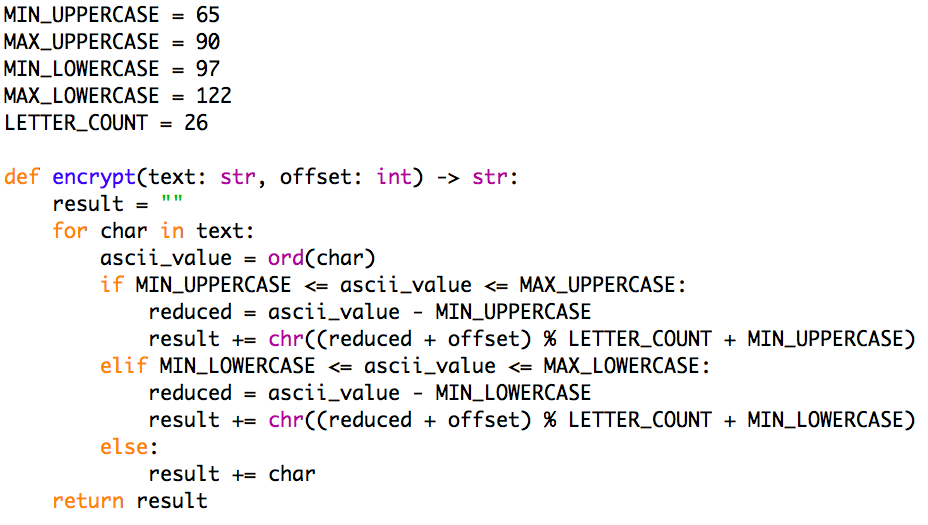
\includegraphics[width=\textwidth]{a1pitfalls/constants}
\end{topic}

\begin{topic}{Alphabet constants}
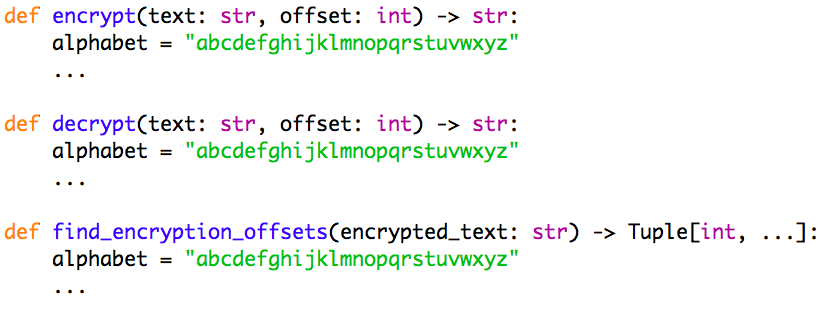
\includegraphics[width=\textwidth]{a1pitfalls/alphabad}
\end{topic}

\begin{topic}{This is better}
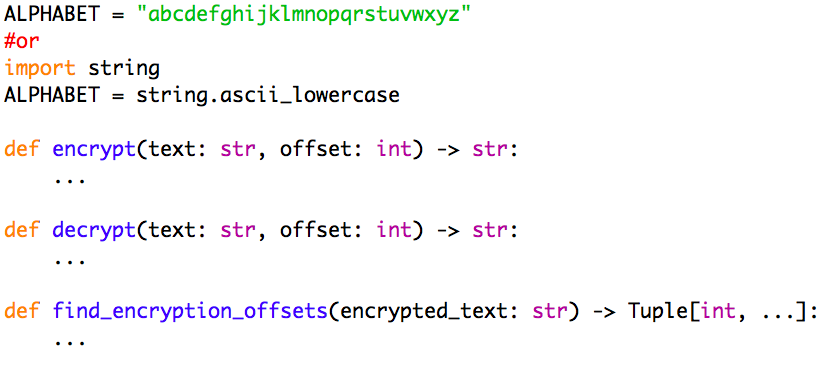
\includegraphics[width=\textwidth]{a1pitfalls/alphagood}
\end{topic}

\begin{topic}{Punctuation checks}
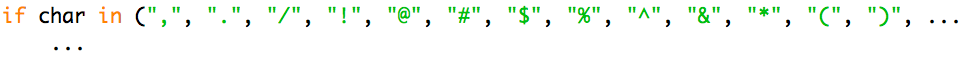
\includegraphics[width=\textwidth]{a1pitfalls/punctubad}
\end{topic}

\begin{topic}{This is better}
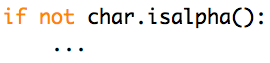
\includegraphics[width=0.5\textwidth]{a1pitfalls/punctugood}
\end{topic}

\begin{topic}{Function definitions}
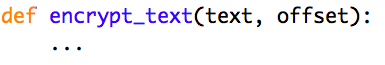
\includegraphics[width=\textwidth]{a1pitfalls/fdef}
\end{topic}

\begin{topic}{Variable naming}
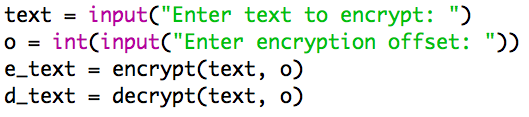
\includegraphics[width=\textwidth]{a1pitfalls/vname}
\end{topic}

\begin{topic}{Other pitfalls}
Handling 0 offset checks in encrypt/decrypt

\begin{subtopic}{2-}
Duplicated code in main (could've split into other functions)
\end{subtopic}

\begin{subtopic}{3-}
Unneccessary casting (eg. \code{text = str(input("enter text"))})
\end{subtopic}

\begin{subtopic}{4-}
Regex (re)
\end{subtopic}

\begin{subtopic}{5-}
Not using the sample tests (or not asking tutors for help with them)
\end{subtopic}

\begin{subtopic}{6-}
Missing out on easy marks by forgetting to write inline comments or not following the docstring guide in the course notes
\end{subtopic}

\end{topic}

\section{Assignment 2 Overview}

\section{Assignment 2 Demo}

\begin{topic}{Assignment 2 Tips}
Review the lecture/tutorial/myPy material on classes/OOP

\begin{subtopic}{2-}
More work than A1, but a lot of trivial methods to write
\end{subtopic}

\begin{subtopic}{3-}
Work on the `easy' marks first - constructors, getters, setters, docstrings
\end{subtopic}

\begin{subtopic}{4-}
Of course... start early ;)
\end{subtopic}
\end{topic}

\end{document} 
